\subsection{Fox}
\begin{figure}[H]
    \centering
    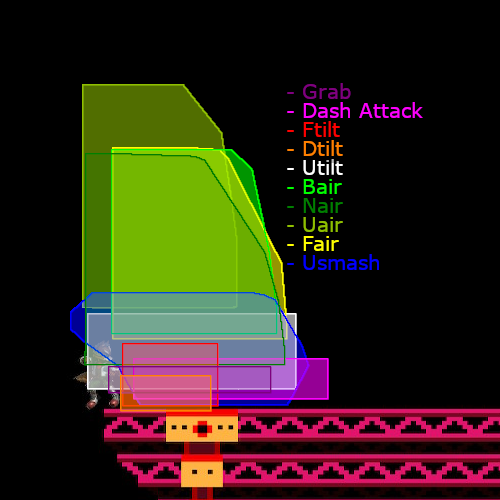
\includegraphics[width=.4\textwidth]{images/threat-ranges/fox}
    \caption{A rough visual of what space Fox can cover in 18 frames\cite{ref:threat-range:fox}}
\end{figure}

\subsection{Pikachu}
\begin{figure}[H]
    \centering
    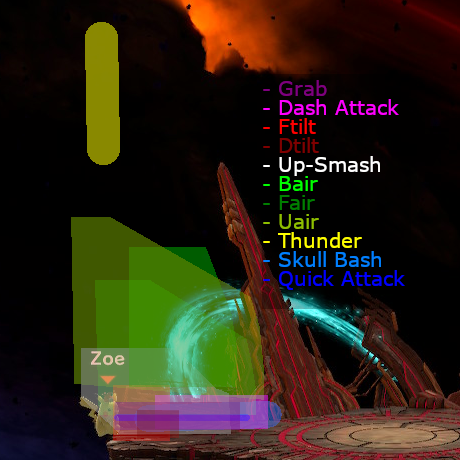
\includegraphics[width=.4\textwidth]{images/threat-ranges/pika}
    \caption{A rough visual of what space Pikachu can cover in 18 frames\cite{ref:threat-range:pika}}
\end{figure}

\subsection{09-luigi.tex}
\subsection{10-ness.tex}
\subsection{Captain Falcon}
\begin{figure}[h]
    \centering
    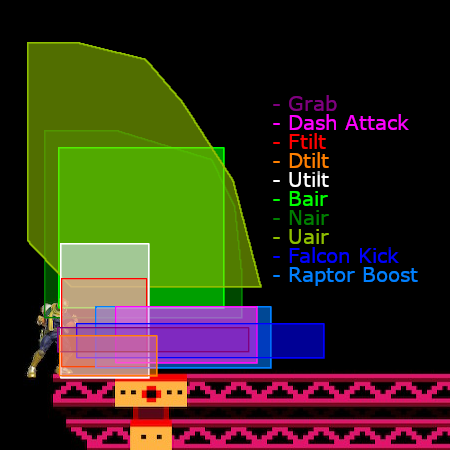
\includegraphics[width=.4\textwidth]{images/threat-ranges/falcon}
    \caption{A rough visual of what space Captain Falcon can cover in 18 frames\cite{ref:threat-range:falcon}}
\end{figure}

\subsection{12-jigglypuff.tex}
\subsection{13-peach.tex}
\subsection{13e-daisy.tex}
\subsection{14-bowser.tex}
\subsection{15-ice-climbers.tex}
\subsection{Sheik}
\begin{figure}[h]
    \centering
    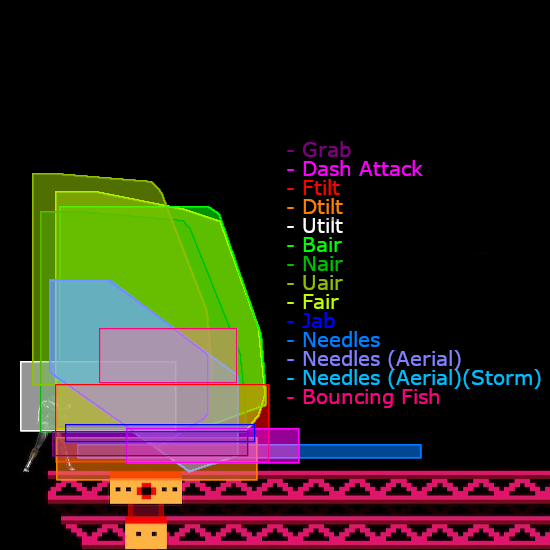
\includegraphics[width=.4\textwidth]{images/threat-ranges/sheik}
    \caption{A rough visual of what space Sheik can cover in 18 frames\cite{ref:threat-range:sheik}}
\end{figure}

\subsection{17-zelda.tex}
\subsection{18-dr-mario.tex}
\subsection{19-pichu.tex}
\subsection{20-falco.tex}
\subsection{21-marth.tex}
\subsection{21e-lucina.tex}
\subsection{22-yink.tex}
\subsection{23-ganon.tex}
\subsection{24-mewtwo.tex}
\subsection{25-roy.tex}
\subsection{25e-chrom.tex}
\subsection{26-gnw.tex}
\subsection{27-mk.tex}
\subsection{28-pit.tex}
\subsection{28e-dark-pit.tex}
\subsection{29-zss.tex}

\subsection{Wario}
\begin{figure}[h]
    \centering
    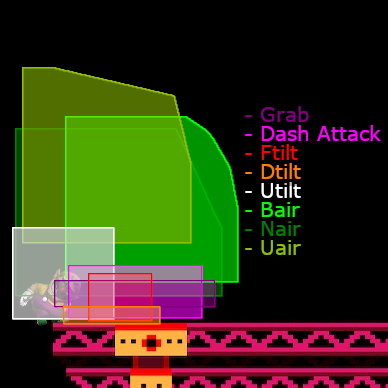
\includegraphics[width=.4\textwidth]{images/threat-ranges/wario}
    \caption{A rough visual of what space Wario can cover in 18 frames\cite{ref:threat-range:wario}}
\end{figure}
\subsection{31-snake.tex}
\subsection{32-ike.tex}
\subsection{33-squirtle.tex}
\subsection{34-ivy.tex}
\subsection{35-charizard.tex}
\subsection{36-diddy.tex}
\subsection{37-lucas.tex}
\subsection{38-sonic.tex}
\subsection{39-ddd.tex}
\subsection{40-olimar.tex}
\subsection{41-lucario.tex}
\subsection{42-rob.tex}
\subsection{43-tink.tex}
\subsection{44-wolf.tex}
\subsection{45-villager.tex}
\subsection{46-megaman.tex}
\subsection{47-wii-fit.tex}
\subsection{48-rosa.tex}
\subsection{49-little-mac.tex}
\subsection{50-greninja.tex}
\subsection{51-brawler.tex}
\subsection{52-swordfighter.tex}
\subsection{53-gunner.tex}
\subsection{54-palu.tex}
\subsection{55-pac-man.tex}
\subsection{56-robin.tex}
\subsection{57-shulk.tex}
\subsection{58-bowser-jr.tex}
\subsection{59-duck-hunt.tex}
\subsection{60-ryu.tex}
\subsection{60e-ken.tex}
\subsection{61-cloud.tex}
\subsection{Corrin}
\begin{figure}[h]
    \centering
    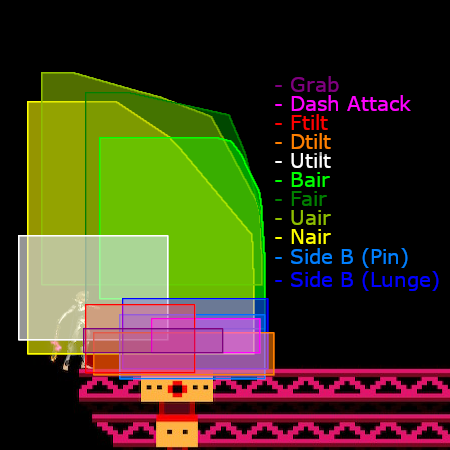
\includegraphics[width=.4\textwidth]{images/threat-ranges/corrin}
    \caption{A rough visual of what space Corrin can cover in 18 frames\cite{ref:threat-range:corrin}}
\end{figure}

\subsection{63-bayo.tex}
\subsection{64-inkling.tex}
\subsection{65-ridley.tex}
\subsection{66-simon.tex}
\subsection{66e-richter.tex}
\subsection{67-krool.tex}
\subsection{68-isabelle.tex}
\subsection{69-incineroar.tex}
\subsection{70-plant.tex}
\subsection{71-joker.tex}
\subsection{72-hero.tex}
\subsection{73-banjo.tex}
\subsection{74-terry.tex}
\subsection{75-byleth.tex}
\subsection{76-min-min.tex}
\subsection{77-steve.tex}
\subsection{78-sephiroth.tex}
\subsection{79-pyra.tex}
\subsection{80-mithra.tex}
\subsection{81-kazuya.tex}
